\pdfminorversion=4
\documentclass{beamer}
\usepackage[utf8]{inputenc}

\usepackage[
backend=biber,
style=alphabetic,
sorting=ynt
]{biblatex}
 
\addbibresource{bibliography.bib}

\usepackage{textcomp}
\usepackage[T1]{fontenc}
\usepackage{multirow}
\usepackage{float}
\usepackage[caption = false]{subfig}
\usepackage{longtable}
\usepackage{listings}
\usepackage{mathtools}
\DeclareMathOperator{\tr}{Tr}
\usepackage{commath}
\usepackage{bbold}
\usepackage{xcolor}
\usepackage{physics}
%\usepackage[margin=1.8cm]{geometry}

\usepackage{tikz-cd} 
\usepackage{amsmath}
\usepackage{amsfonts}
\usepackage{amssymb}
\usepackage{amsthm}
\usepackage{graphicx}
\usepackage[colorinlistoftodos]{todonotes}
\usepackage[colorlinks=true, allcolors=blue]{hyperref}
\usepackage{siunitx}
\sisetup{separate-uncertainty=true}

\usepackage[sc]{mathpazo}
\linespread{1.05}         % Palladio needs more leading (space between lines)
\usepackage[T1]{fontenc}

\newcommand{\diag}[1]{\text{diag}\qty(#1)}
\newcommand{\Lagr}{\mathcal{L}}
\newcommand{\const}{\text{const}}
\newcommand{\sign}[1]{\text{sign}\qty(#1)}
\usetheme{Rochester}
% \usepackage[scaled]{helvet} % ss

\title{Relativistic Non-Ideal Flows}
\author{Laureando: Jacopo Tissino \\
    Relatore: prof.\ Roberto Turolla}
\date{24/09/2019}

\begin{document}

\frame{\titlepage}

\begin{frame}
    \frametitle{The Schwarzschild metric}
    Flat metric:

    \begin{equation*}
        \dd{s}^2 = -\dd{t}^2 + \dd{r}^2 + r^2 \qty(\dd{\theta}^2 + \sin^2\theta \dd{\varphi})\,.
    \end{equation*}

    Schwarzschild metric:

    \begin{equation*}
        \dd{s}^2 = -\qty(1-\frac{2M}{r})\dd{t}^2 + \frac{1}{1-\frac{2M}{r}} \dd{r}^2
        + r^2 \qty(\dd{\theta}^2 + \sin^2\theta \dd{\varphi})\,,
    \end{equation*}
    %
    where \(c = G = 1\).

    % The radial coordinate \(r\) can be defined with the 2-sphere's area: \(A \overset{!}{=} 4 \pi r^2\) since the angular metric is flat.

    % The singularity at \(r = 2M \) is not physical: there are other coordinates in which it disappears and the physical behaviour is revealed, objects \emph{can} actually reach the horizon in finite time.
\end{frame}

\begin{frame}
    \frametitle{The Schwarzschild metric}
    \begin{figure}
        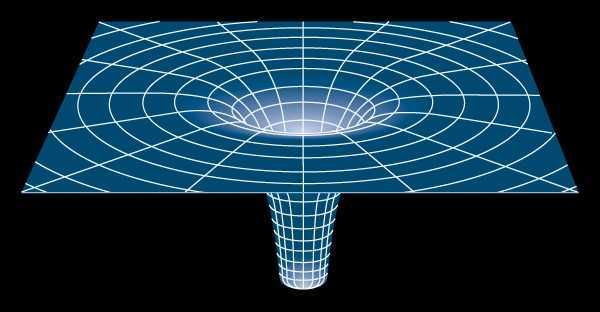
\includegraphics[width=\textwidth]{figures/Schwarzschild-Space}
    \end{figure}

    {\tiny Image credit: \url{https://www.physicsforums.com/insights/schwarzschild-metric-part-1-gps-satellites/}.}

    % Circles are spaced further apart on the manifold than their radii's difference
\end{frame}


\begin{frame}
    \frametitle{Tetrads: the Local Rest Frame}

    A tetrad is a set of vectors \(V^\mu _{(\alpha)}\) which are Fermi-Walker transported and satisfy:
    %
    \begin{equation*}
        g_{\mu\nu} V^\mu _{(\alpha)} V^\nu _{(\beta)} = \eta_{(\alpha) (\beta)}\,.
    \end{equation*}

    If we assume spherical symmetry and stationarity, we can determine the whole tetrad if we have the normalized radius \(r/2M\) and the velocity \(v\).
\end{frame}

\begin{frame}
    \frametitle{The Local Rest Frame}
        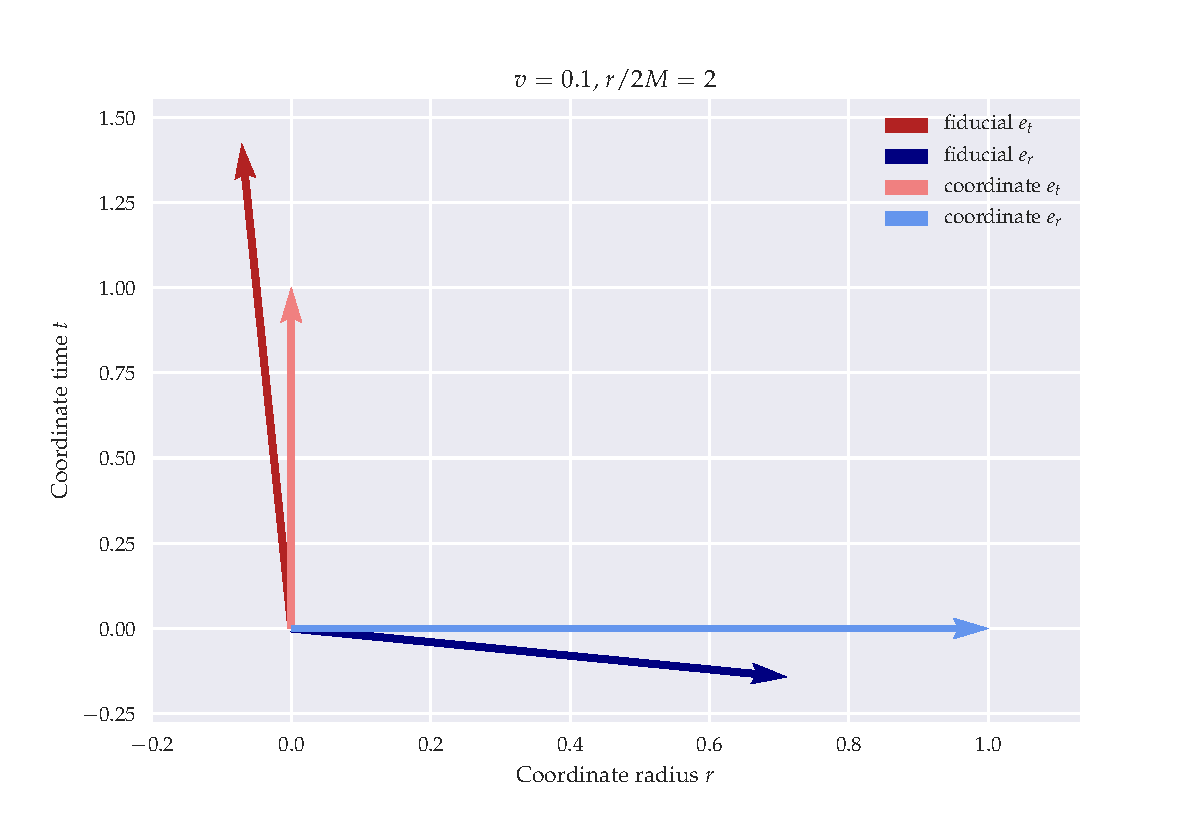
\includegraphics[width=\textwidth]{figures/low_speed}
\end{frame}

\begin{frame}
    \frametitle{The Local Rest Frame}
        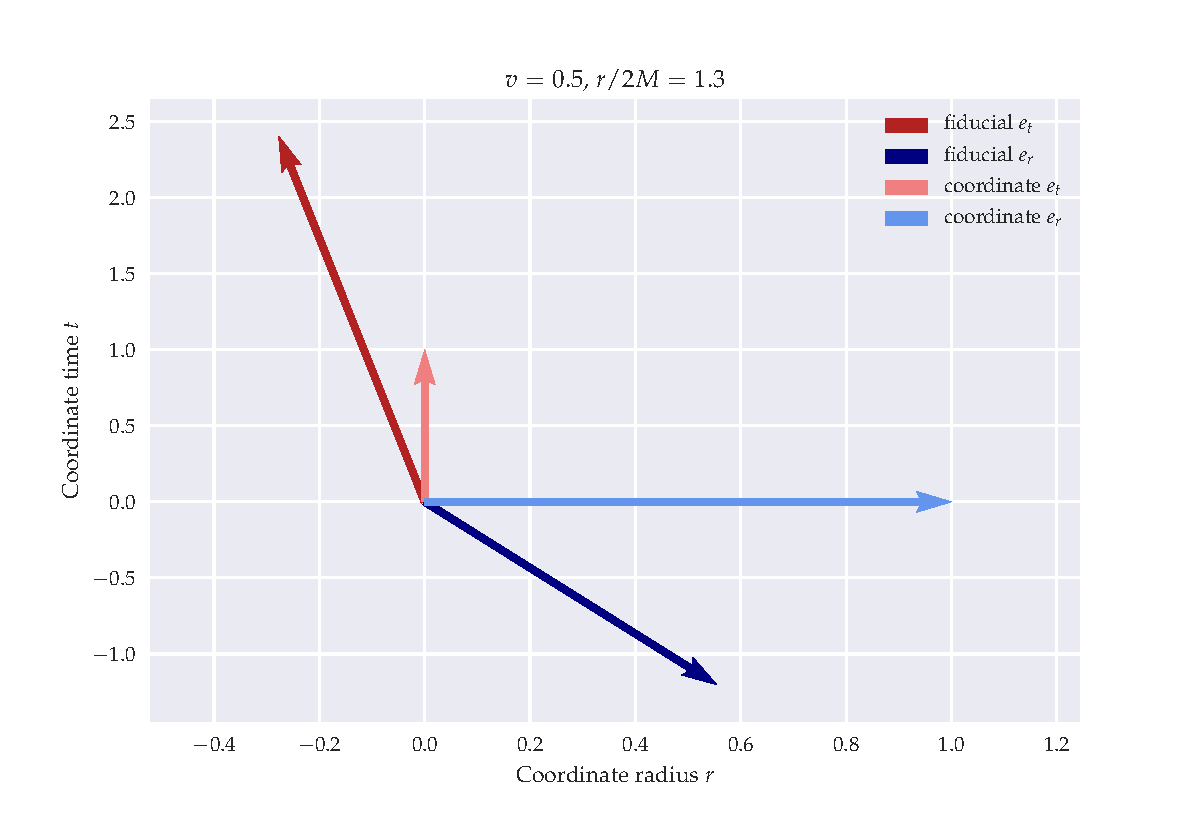
\includegraphics[width=\textwidth]{figures/high_speed}
\end{frame}

\begin{frame}
    \frametitle{The stress-energy tensor}

    The component \(T^{\mu\nu}\) is the flux of \(\mu\)-th component of the four-momentum \(p^\mu\) through a surface of constant coordinate \(x^\nu\).

    For an ideal fluid (\(\eta = \xi = \kappa = 0\)) in the Local Rest Frame:

    \begin{equation*}
        T^{\mu\nu}_{\text{ideal fluid}} =
        \begin{bmatrix}
        \rho   &   &   &  \\
           & p  &   &  \\
           &   & p  &  \\
           &   &   & p
       \end{bmatrix}_{\text{fid}} \,,
    \end{equation*}
    %
    where \(\rho = \rho_0 (1 + \varepsilon)\).
\end{frame}

\begin{frame}
    \frametitle{The radiation moments}

    \begin{subequations}
    \begin{align*}
      w_0 &= \int I \dd{\Omega} & \text{radiation energy density} \\
      w_1 &= \int I \cos \theta \dd{\Omega} & \text{radiation energy flux} \\
      w_2 &= \int I \qty(\cos^2 \theta - \frac{1}{3}) \dd{\Omega} & \text{radiation shear stress.}
    \end{align*}
    \end{subequations}
\end{frame}

\begin{frame}
    \frametitle{The radiation moments}

    \incfig{figures/moments}
\end{frame}

\begin{frame}
    \frametitle{The full stress-energy tensor}

    \begin{equation*}
    T^{\mu\nu} =
    T^{\mu\nu}_{\text{ideal fluid}} +
    \begin{bmatrix}
    w_0   & w_1  & 0  & 0 \\
    w_1   & \frac{1}{3}w_0 + w_2  &  0  & 0 \\
      0 & 0  &  \frac{1}{3}w_0 -\frac{1}{2}w_2 & 0 \\
      0 & 0  &  0 & \frac{1}{3}w_0 -\frac{1}{2}w_2
    \end{bmatrix} _{\text{fid}}
    \end{equation*}

    The equations to solve are:

    \begin{subequations}
    \begin{align*}
      \nabla_\mu T^{\mu\nu} = 0 && \text{2 equations} \\
      \nabla_\mu \qty(\rho_0 u^\mu) = 0&& \text{1 equation} \\
      \text{conservation of photon number} && \text{2 equations.}
    \end{align*}
    \end{subequations}
\end{frame}

\begin{frame}
    \frametitle{Singularities}
    There is a singularity in the Euler equation at \(v = v_s\):
        \begin{equation*}
        (v^2 - v_s^2) \frac{(yv) ^{\prime}}{yv} - 2 v_s^2 + \frac{M}{y^2 r}
        = -\frac{r}{yv (p + \rho)} \qty((\Gamma-1)s_0 + v s_1)\,.
        \end{equation*}
        %
    Also, since we assume \(w_2 = f(\tau) w_1\), there is another singularity at the zeroes of:
    %
    \begin{equation*}
        v^2 - v f(\tau) - \frac{1}{3}
    \end{equation*}
\end{frame}

\begin{frame}
    \frametitle{Accretion efficiency}
    The Eddington luminosity is attained when the radiation pressure on a test hydrogen atom equals the gravitational pull on it. We have approximately:

    \begin{equation*}
        \frac{L_{\text{Edd}}}{M} = \frac{4 \pi c G m_p}{\sigma_T} \approx \num{3.27e4} \frac{L_{\odot}}{M_{\odot}}  \,.
    \end{equation*}

    From the fit, fixing \(\dot{M}\), we get \(L = 4 \pi r^2 w_1\).

    We look at \(l = L / L_{\text{Edd}}\) in terms of \(\dot{m} = \dot{M} c^2 / L_{\text{Edd}}\).
\end{frame}

\begin{frame}
    \frametitle{Accretion efficiency}
    \centering
    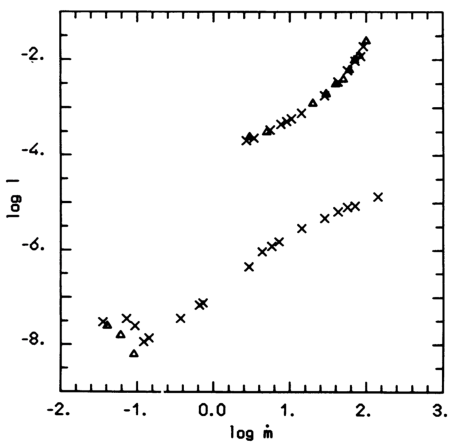
\includegraphics[width=0.7\textwidth]{../figures/logl-logm}
\end{frame}

\end{document}
